\chapter{The effects of varying depth}
\label{sec:eff_of_var_depth}
In this chapter we will explore the effects of varying depth on different shear statistics. In abstract terms, this is a position-based selection effect: In some places fainter galaxies can not be detected due to higher noise levels, whereas in other places the same galaxies would be detected. This leads to a modification of number density, as in deeper pointings more galaxies can be detected, as well as a modification in the shear statistics themselves, as fainter galaxies are on average located at a higher redshift.

We will be working with data from the KiDS+Viking-450 (KV450) Survey \citep{2018arXiv181206077W}. The KV450 survey combines data in the $ugri$-band from the Kilo Degree Survey (KiDS) with the $ZYJHK_{\rm s}$-band imaging from the VISTA Kilo Degree Infrared Galaxy Survey (VIKING) over 458 square degrees. The unprecedented coverage in 9 photometric bins allows a relatively narrow photometric-to-spectroscopic redshift comparison and thus significanlty reduces systematic biases arising from incorrect redshift determination.

For the cosmic shear analysis, the galaxies were separated into five tomographic bins of photometric redshift $z_{\rm b}$. In the areas where the survey overlaps with spectroscopic surveys, a true redshift distribution was extracted for each of the tomographic bins. A summary of the bin boundaries, the (weighted) number of galaxies\footnote{Throughout this thesis, when we speak of the (weighted) number of galaxies in a sample, we refer to the sum of all lensing weights of the galaxies belonging to the respective sample. As all quantities like the average redshift distribution, the shear correlation functions etc.\! are calculated using this number, it carries way more information than the unweighted number of galaxies. For that reason, whenever we speak of a number of galaxies, unless otherwise specified, we refer to the sum of their respective lensing weights.} in each bin and the average spectroscopic redshifts can be found in Table \ref{tab:tomograpic_bins}. A detailed explanation of the determination of the redshift distributions, the measured correlation functions and the inferred cosmological parameters can be found in \citet{2017MNRAS.465.1454H,2018arXiv181206076H}.
\begin{SCtable}
\centering
\begin{tabular}{ccccc}
\toprule
Bin & $z_{\rm b}^{\rm{min}}$ & $z_{\rm b}^{\rm{max}}$ & $N$ & $\la z_{\rm{spec}} \ra$ \\
\midrule
1 & 0.1 & 0.3 &   386208 & 0.49 \\
2 & 0.3 & 0.5 &   563719 & 0.53 \\
3 & 0.5 & 0.7 &   799492 & 0.69 \\
4 & 0.7 & 0.9 &   532226 & 0.84 \\
5 & 0.9 & 1.2 &   415980 & 1.00 \\
\bottomrule
\end{tabular}
\caption[Properties of the tomographic redshift bins in the KV450 Survey.]{Minimum photometric redshift $z_{\rm b}^{\rm{min}}$, maximum photometric redshift $z_{\rm b}^{\rm{max}}$, weighted number of galaxies $N$ and average spectroscopic redshift  $\la z_{\rm{spec}} \ra$ of the five tomographic redshift bins in the KV450 Survey.}
\label{tab:tomograpic_bins}
\end{SCtable}
\begin{figure}
\centering
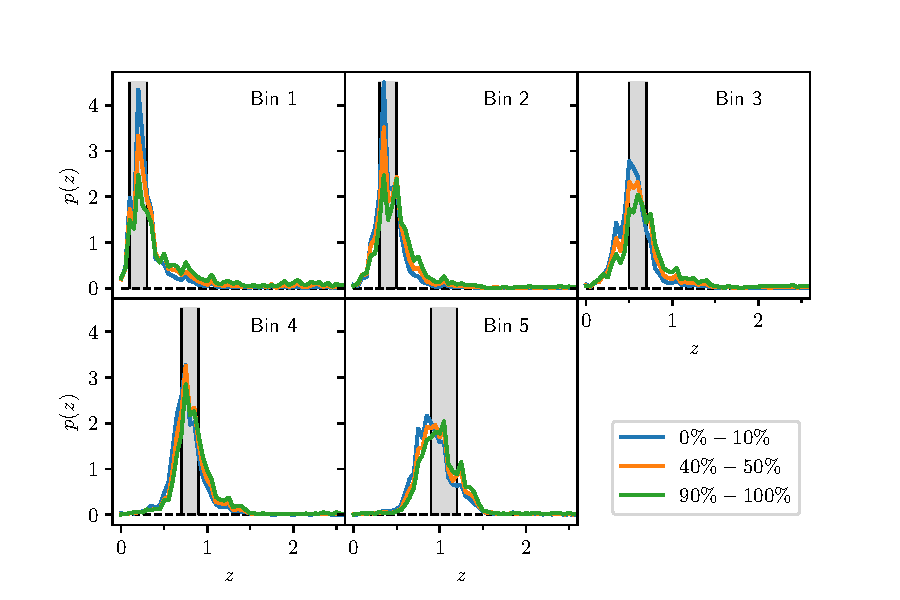
\includegraphics[trim={0.5cm 0 1cm 0},clip,width=\textwidth]{dist_z_all.pdf}
\caption[Redshift distribution for the worst, a medium and the best percentile]{Redshift distribution for the worst, a medium and the best percentile for each tomograpic bin. The grey area highlights photometric redshift bin.}
\label{fig:redshifts_per_percentile}
\end{figure}

While there are many position-based selection effects having similar impacts, like depth in the different colour bands, seeing, airmass, Galactic extinction, dithering strategies and CCD imperfections, we chose to focus on the $r$-band depth of a pointing. As the $r$-band served as the detection band, its depth appears to be the most relevant factor. As of now, we ignore the other effects as we expect them to play a subdominant role, but the investigation of those is definitely necessary in further studies.

To estimate the extent of the varying depth between pointings, we received some data by H.~Hildebrandt: All pointings were sorted by $r$-band depth and split into ten percentiles, ordered from shallow to deep. For each of the percentiles of every tomographic bin, the redshift distribution and the weighted number of galaxies were extracted. Inspecting Figure \ref{fig:redshifts_per_percentile}, one can clearly see that the redshift distribution strongly varies between the percentiles -- especially the lower-redshift bins show a significant tail of high-redshift galaxies for deep pointings. It is also noticeable that the spectroscopic redshift distribution of galaxies only roughly traces their photometric redshift bins. While this might seem like a problem, as long as we have a precise knowledge the spectroscopic redshift distribution for Eq.\,\eqref{eq:pkappa}, this does not affect the results. 

\begin{figure}
\centering
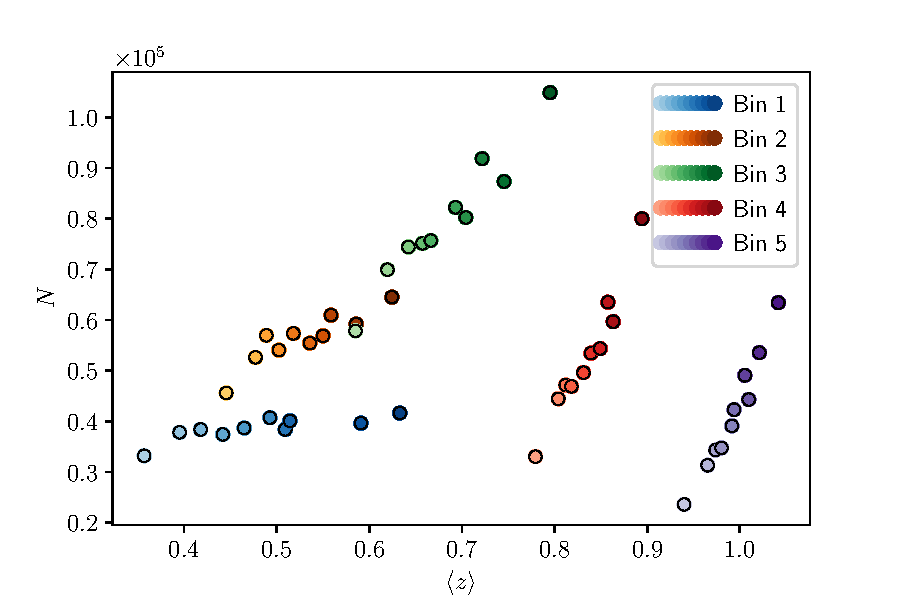
\includegraphics[width=0.8\linewidth]{cov_nz_meanz.pdf}
\caption[Weighted number of galaxies as a function of redshift]{Weighted number of galaxies $N$ as a function of average (spectroscopic) redshift $\la z \ra$ for each percentile of the five tomographic bins. Values for this can be found in Table \ref{tab:nvsz} in the Appendix.}
\label{fig:number_density_vs_redshift}
\end{figure}

Additionally, when we look at Figure \ref{fig:number_density_vs_redshift}, we notice some interesting features: First and foremost, there is an obvious strong correlation between average redshift and the number of galaxies for all bins. Furthermore, the low redshift bins seem to vary extremely strongly in redshift and only subdominantly in the number of galaxies, whereas the trend is vice versa for the high-redshift bins. This behaviour is easily explained: Almost all galaxies in the low-redshift bins are close (and thus bright) enough for us to detect them, even with suboptimal depth in the pointing. A significant fraction of the galaxies included in the high percentiles are ones with extremely high ($z \gtrsim 2$) spectroscopic redshift, which leads to a strong increase in average redshift. The galaxies in the high-redshift bins, however, are relatively dim and thus harder to detect. For shallow pointings the number of detected galaxies thus significantly decreases. Still, the additional galaxies detected in deeper pointings do not influence the average redshift that much, as the average redshift is already pretty high.

We see that the $r$-band depth has a strong effect on the number of detected galaxies as well as on their average redshift. These two effects will definitely influence the measured shear statistics if one does not account for them. In the next two sections we will develop a few models to help us answer the question whether this influence is significant for the results of the KV450 survey, and if it can be detected by analysis of the B-modes.
\section{Toy model -- a single lens plane}
\label{sec:toy_model}
For our first analysis we will further simplify our assumptions: We imagine that all the matter between sources and observer is concentrated in a single lens plane of distance $D_{\rm d}$ from the observer. If we now distribute sources at varying distances $D_{\rm s}$, then the convergence $\kappa$ varies according to $\kappa \propto \Dds/D_{\rm s}$. 

Assuming that the survey depth, and thus the source redshift populations, vary between pointings, an observer will measure a shear-signal that is modified by a depth function $W(\bm{\theta}) = 1+w(\bm{\theta})\propto \Dds/D_{\rm s}$, where $\langle w(\bm{\theta})\rangle=0$ holds. We will model the effects of such a depth function in three different ways - by modelling a convergence field directly, by computing the effects on the power spectrum and by investigating the change of the shear correlation functions.

\subsection{Modelling a shear field}
\label{sec:model_kappa}
As a first test, we simulated the convergence $\kappa$ as a Gaussian random field\footnote{A Gaussian random field is fully characterized by its power spectrum $P(|\b k|)$. A particular realization is obtained by drawing Gaussian deviates with dispersion $\sigma(\b k)=\sqrt{P(|\b k|)}$ for each $\b k$, multiplying them with a random phase $\phi_{\b k}$, and then Fourier transforming the obtained field.} and converted it to a shear-field $\gamma$ via Eq.\,\eqref{eq:KS_gamma_from_kappa}. This field was then multiplied by a pointing-based depth function $W(\b\theta)$. For simplicity we modelled the weighting by random variables from a normal distribution with mean $\mu = 1$ and variance $\sigma = 0.1$. After that, we transformed the shear field back into a convergence field $\kappa^{\rm{obs}}$. The transformations between the fields were done using the convolution theorem. For the Fourier transformations, periodic boundary conditions were asserted. As the observed shear field is modified, the reconstruction of the observed convergence $\kappa^{\rm{obs}}$ will not yield the original convergence. In particular, there is no reason why the convolution with a complex kernel should have a nonzero imaginary part. This allows us to separate our received signal into E- and B-modes via Eq.\,\eqref{eq:ebmodes1}. As an example, Figure \ref{fig:way_for_kappa} shows the procedure for one $4\times 4\,\rm{deg}^2$-field.
\begin{figure}
\centering
\begin{subfigure}[c]{0.49\textwidth}
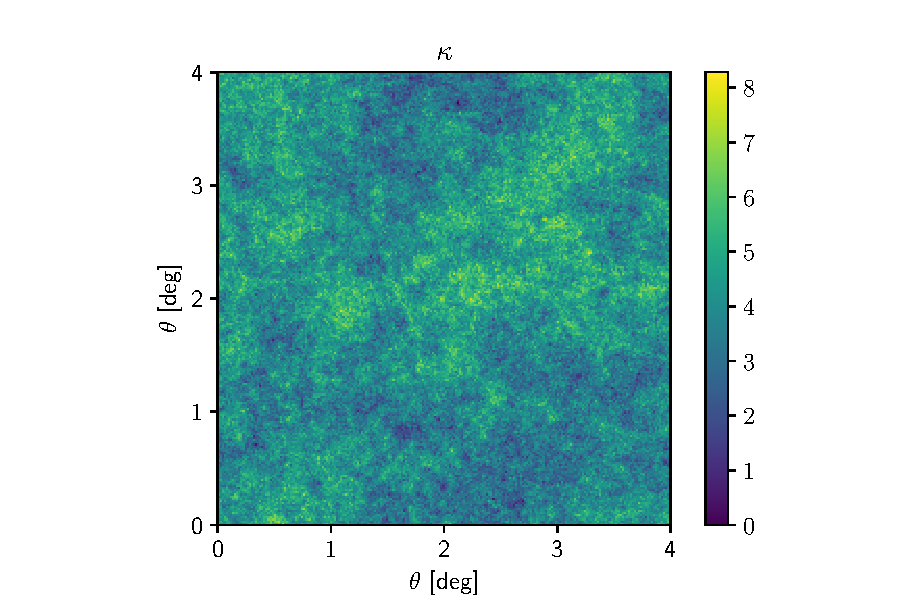
\includegraphics[trim={1.2cm 0cm 1.2cm 0cm},clip,width=\textwidth]{kappa.pdf}
\subcaption{Initial convergence $\kappa$.}
\end{subfigure}
\begin{subfigure}[c]{0.49\textwidth}
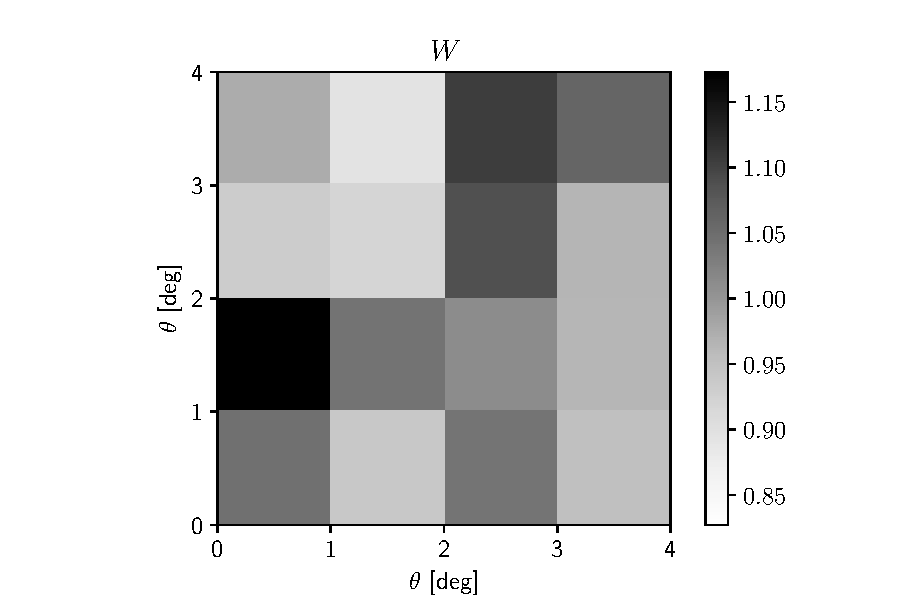
\includegraphics[trim={1.2cm 0cm 1.2cm 0cm},clip,width=\textwidth]{weightf.pdf}
\subcaption{Used weight-function $W$.}
\end{subfigure}\\
\begin{subfigure}[c]{0.49\textwidth}
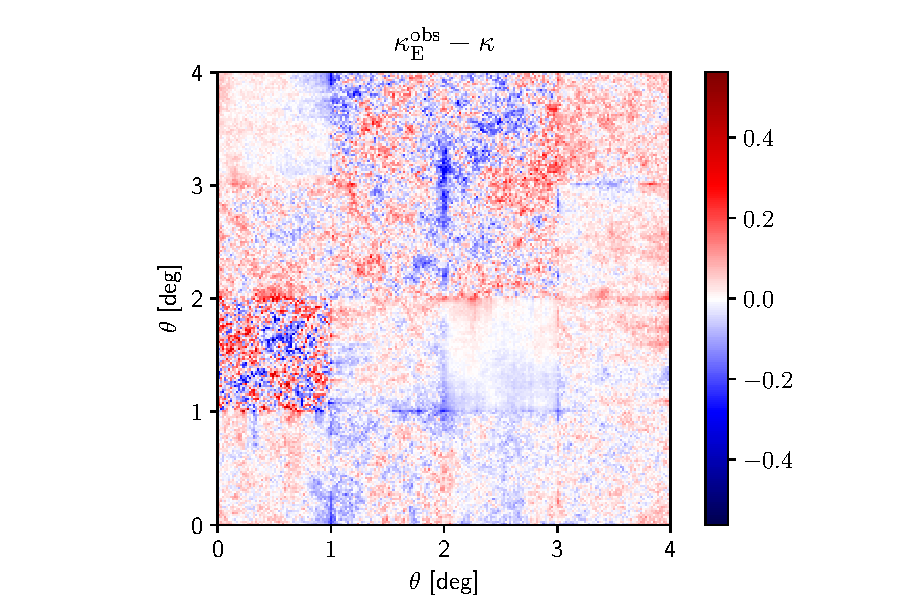
\includegraphics[trim={1.2cm 0cm 1.2cm 0cm},clip,width=\textwidth]{kappae.pdf}
\subcaption{Difference in E-modes between the initial convergence field $\kappa$ and the reconstructed convergence field $\kappa^{\rm{obs}}$.}
\end{subfigure}
\begin{subfigure}[c]{0.49\textwidth}
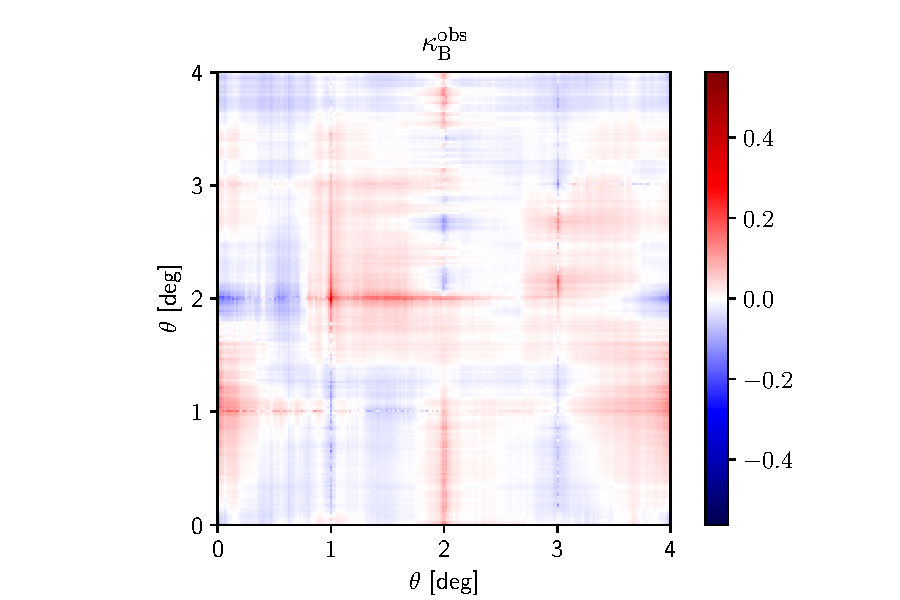
\includegraphics[trim={1.2cm 0cm 1.2cm 0cm},clip,width=\textwidth]{kappab.pdf}
\subcaption{B-modes of the reconstructed convergence field $\kappa^{\rm{obs}}$.}
\end{subfigure}
\caption{Estimating E- and B-modes of a reconstructed convergence field.}
\label{fig:way_for_kappa}
\end{figure}

It is interesting to note that the difference in E-modes is predominantly within the $1\,\rm{deg}^2$-fields, whereas the majority of B-modes arise close to the boundaries of each field. However, the reconstructed convergence field is not a good statistic for cosmic shear. Additionally, while the initial density fluctuations might be a Gaussian random field, cosmic shear is measured in the nonlinear regime of structure growth, which no longer takes the form of a Gaussian random field. While this visual inspection serves as a good first start, it is not suitable to make any reliable predictions. For this reason, I chose to investigate two-point shear statistics, namely the power spectrum and the shear correlation functions.
%where $B$-Modes can not be generated by a lensing signal and are thus a tracer of remaining systematics.
%2002A&A...389..729S SRC
\subsection{Effects on the power spectrum}
\label{sec:model_ps}
For the analysis of the power spectrum we adopt the same pointing-based depth function \linebreak$\gammao(\b\theta)=W(\b \theta)\gamma(\b\theta)$ with $W(\bm{\theta}) = 1+w(\bm{\theta})$, where $\langle w(\bm{\theta})\rangle=0$ holds. 
In accordance to the definition of the shear power spectrum \begin{equation}
(2\pi)^2\delta(\b\ell-\b\ell')P(|\b\ell|) = \la \tilde{\gamma}(\b\ell)\tilde{\gamma}(\b\ell')\ra \, ,
\end{equation}
we define the observed power spectrum via \begin{equation}
P^{\text{obs}}(\b\ell) \equiv \frac{1}{(2\pi)^2}\int \d^2 \ell'\,  \la \gammaoh(\b \ell) \gammaoh {}^*(\b \ell')\ra \, .
\end{equation}
Note that due to the depth-function both the assumptions of homogeneity and isotropy break down, which means that we can neither assume isotropy in the power spectrum, nor can we assume that $\la \gammaoh(\b \ell) \gammaoh {}^*(\b \ell')\ra$ vanishes for $\b\ell\neq\b\ell'$. In this section we will outline the computation of the observed power spectrum. A more detailed version can be found in Appendix \ref{sec:calc of PS}. We compute the correlation of the Fourier transformed observed shear as \begin{align*}
\la \gammaoh(\b \ell) \gammaoh {}^*(\b \ell')\ra = & \la\int\text{d}^2 \theta\int\text{d}^2 \theta'\,W(\b \theta)W(\b \theta')\gamma(\b \theta)\gamma^*(\b \theta')\exp(\i\b \ell\cdot\b \theta-\i\b \ell'\cdot\b \theta')\ra \nonumber \\
  = & \la \int\frac{\text{d}^2 \b k}{(2\pi)^2} \, P(\b k)\widetilde{W}(\b \ell-\b k)\widetilde{W}^* (\b \ell'-\b k)\ra \, .
\end{align*}
Inserting $W(\b\theta) = 1+w(\b\theta)$ we derive \begin{align*}
\la \gammaoh(\b \ell) \gammaoh {}^*(\b \ell')\ra = & \la \int\frac{\text{d}^2 k}{(2\pi)^2} \, P(\b k) \left[ (2\pi)^4\delta(\b \ell-\b k)\delta(\b \ell'-\b k)+(2\pi)^2\big[ \tilde{w}(\b \ell-\b k)\delta(\b \ell'-\b k)\right.\right. \nonumber\\
 & \qquad \left.\left.  + \tilde{w}^*(\b \ell'-\b k)\delta(\b \ell-\b k)\big]+ \tilde{w}(\b \ell-\b k)\tilde{w}(\b \ell'-\b k) \right] \right. \bigg> \nonumber\\
= & (2\pi)^2\delta(\b \ell-\b \ell')P(\b \ell) + \la \int \frac{\text{d}^2 k}{(2\pi)^2}\, \tilde{w}(\b \ell-\b k)\tilde{w}^*(\b \ell'-\b k)P(\b k)\ra \, .
\end{align*}
To model an arbitrary depth function that is constant on each individual pointing $\b \alpha$, we can choose weights $w_{\b \alpha}$, that only need to satisfy $\langle w_{\b \alpha}\rangle=0$, and parametrize $w(\b\theta)$ as 
\begin{equation}
w(\b \theta) = \sum_{\b \alpha \in \mathbb{Z}^2} w_{\b \alpha} \Xi(\b \theta-L\b \alpha)\text{ , with the Box-Function } \Xi(\b \theta) = \begin{cases}
1 \qquad \b \theta\in \left[-\frac{L}{2},\frac{L}{2}\right]^2 \\
0 \qquad \text{else}
\end{cases},
\label{eq:defweightf}
\end{equation}
where $L$ is the length of one pointing.  Assuming an uncorrelated distribution for the weight function $\left(\la w_{\b\alpha}w_{\b\beta}\ra =0\text{ for }\b\alpha\neq\b\beta\right)$, we define $\la w^2\ra\equiv\la w_{\b\alpha}^2\ra$. We can then calculate the observed power spectrum via
\begin{align}
P^{\text{obs}}(\b \ell)  = & \frac{1}{(2\pi)^2}\int\d^2\ell' \la \gammaoh(\b \ell) \gammaoh {}^*(\b \ell')\ra\nonumber\\
  = & P(\b \ell) + \la w^2\ra \int\frac{\text{d}^2 k}{(2\pi)^2}\,\widetilde{\Xi}(\b \ell-\b k)P(\b k)\, ,
\end{align}
where $\widetilde{\Xi}$ is the Fourier transform of a box-function, namely a sinc-function.

The observed power spectrum $P^{\text{obs}}$ is thus composed of the original power spectrum $P$, plus a convolution of the power spectrum with a two-dimensional sinc-function, scaling with the variance of the geometric lensing efficiency $\la \frac{D_{\rm ds}}{D_{s}}\ra$. In particular, the power spectrum is not isotropic anymore. Following \citet{2002A&A...389..729S}, it would be interesting to extract E- and B-mode information out of this power spectrum. The B-mode power spectrum for the simulations described in Section \ref{sec:model_kappa}, this time for a $20\times 20\,\rm{deg}^2$-field, can be seen in Figure \ref{fig:powerspectra}. As the B-mode power spectrum is solely created by this effect, the imprint of the sinc-function is clearly visible.

\begin{figure}
\begin{subfigure}[c]{0.49\textwidth}
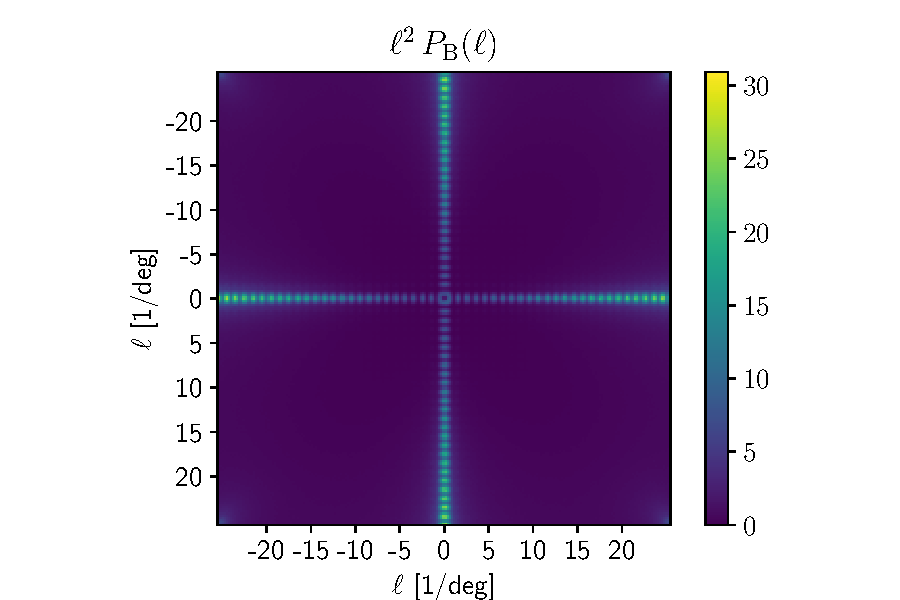
\includegraphics[trim={1.2cm 0cm 1.2cm 0cm},clip,width=\textwidth]{pp3_2.pdf}
\subcaption{Two-dimensional B-mode power spectrum.}
\end{subfigure}
\begin{subfigure}[c]{0.49\textwidth}
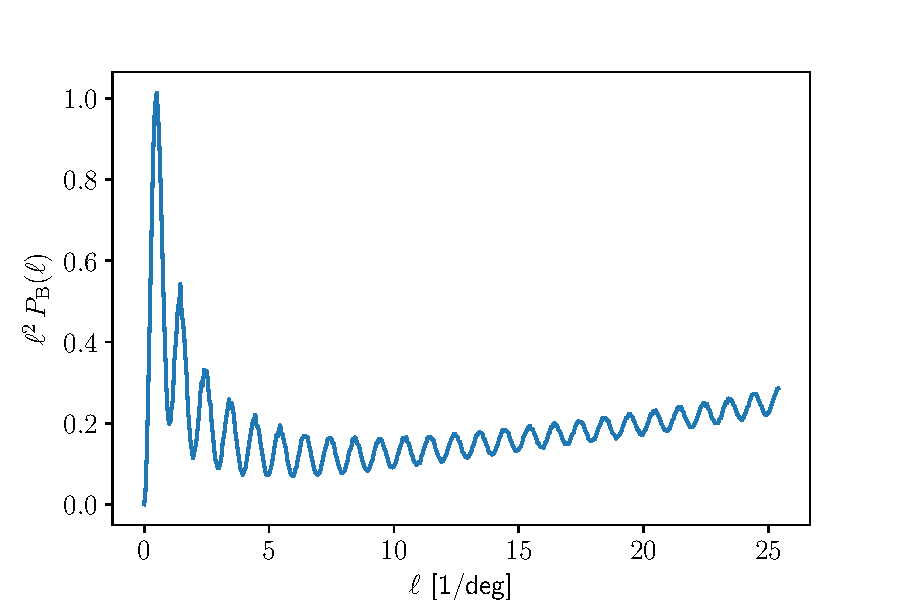
\includegraphics[trim={0.2cm 0cm 1.2cm 0cm},clip,width=\textwidth]{pkappa2i.pdf}
\subcaption{Azimuthally averaged B-mode power spectrum.}
\end{subfigure}
\caption[B-mode power spectra in Gaussian random fields]{One- and two-dimensional B-mode power spectra for simulations of Gaussian random fields.}
\label{fig:powerspectra}
\end{figure}

Unfortunately, it is quite difficult to include any form of weighting in the analysis of the power spectrum, both in the form of number density and in the form of lensing weights. We will therefore analyse the change in the shear correlation functions, as these functions allow for a straightforward implementation of weightings. For the E- and B-mode decomposition we will rely on the COSEBIs \citep{2010A&A...520A.116S}.
\subsection{The function $E(\theta)$}
\label{sec:model_e}
When computing the shear correlation between a pair of galaxies, it is of central importance whether those two galaxies lie in the same pointing or not. We want to model the probability that a pair of galaxies with separation $\b\theta$ lie in the same pointing by the function $E(\b\theta)$, which we will derive here:

{
\def\vec{\b}
\begin{SCfigure}
    \centering
    \def\svgwidth{200pt}    
    \hspace*{1cm}
    \input{../figs/eoftheta_new.pdf_tex}  
    \hspace*{-2cm}
    \caption[Graphic how to obtain $E(\b\theta)$]{Graphic representation on how to obtain the function $E(\b\theta)$. For a separation vector $\b\theta$, the dashed square represents the area of galaxies that have their partner in the same pointing.}
    \label{fig:explain_etheta}
\end{SCfigure}
}
Given one square field of length $L$ (in our case $L=60\arcmin$) and a separation vector $\b\theta$, without loss of generality we can assume $\theta_1,\theta_2\geq 0$. As depicted in Figure \ref{fig:explain_etheta}, the dashed square represents all possible positions that the first galaxy can take, such that the second galaxy is still within the same pointing. The volume of this square equals \begin{equation}
V(|\b\theta|,\phi)  = \big[L-|\b\theta|\cos(\phi)\big]\,\big[L-|\b\theta|\sin(\phi)\big]\, ,
\end{equation} where $\phi$ represents the angle of the vector $\b\theta$. The function $E(\b\theta)$ then simply equals $V(|\b\theta|,\phi)/L^2$. To exclude negative Volumes (which could occur when $|\b\theta|>1$ holds), we need to add the Heaviside theta function $\mathcal{H}$:
\begin{equation}
E(\b\theta)  = \left[1-\frac{|\b\theta|}{L}\cos(\phi)\right]\,\left[1-\frac{|\b\theta|}{L}\sin(\phi)\right]\, \mathcal{H}\left[1-\frac{|\b\theta|}{L}\cos(\phi)\right]\,\mathcal{H}\left[1-\frac{|\b\theta|}{L}\sin(\phi)\right]\, .
\label{eq:eoftheta1}
\end{equation} 
As $E(\b\theta)$ is not isotropic, in order to obtain the function $E(\theta) = E(|\b\theta|)$, we need to azimuthally average Equation \eqref{eq:eoftheta1} over all angles $\phi$. While the case $\theta_1,\theta_2\geq 0$ certainly does not hold for all angles $\phi$, we can eliminate the other cases by simple symmetry.
\begin{align}
E(\theta) = & \frac{4}{2\pi}\int_0^{\frac{\pi}{2}}\d\phi\, E(\b\theta) = \frac{2}{\pi}\begin{cases}
\int_0^{\frac{\pi}{2}} \d\phi\, \left[1-\frac{|\b\theta|}{L}\cos(\phi)\right]\,\left[1-\frac{|\b\theta|}{L}\sin(\phi)\right]\, ,  & |\b\theta|  \leq L \\[10pt]
\int_{\cos\inv(L/|\b\theta|)}^{\sin\inv(L/|\b\theta|)} \d\phi\, \left[1-\frac{|\b\theta|}{L}\cos(\phi)\right]\,\left[1-\frac{|\b\theta|}{L}\sin(\phi)\right] \, , \quad   & L \leq |\b\theta| \leq \sqrt{2}L \\[10pt]
0\, , &\sqrt{2}L \leq\theta
\end{cases} \nonumber\\[10pt]
 = & \begin{cases}
\frac{1}{L^2 \pi}\left[L^2\pi - (4L-\theta) \theta\right]\, ,  & \theta \leq L \\[10pt]
\frac{2}{\pi}\,\left[4\sqrt{\frac{\theta^2}{L^2}-1} -1 - \frac{\theta^2}{2L^2} - \cos\inv\left(\frac{L}{\theta}\right) + \sin\inv\left(\frac{L}{\theta}\right)\right]\, ,  & L  \leq \theta \leq \sqrt{2}L \\[10pt]
0\, ,  & \sqrt{2}L \leq \theta
\end{cases}\, .
\end{align}

The function is depicted in Figure \ref{fig:eoftheta_lin}. 
 
 \begin{figure}
 \centering
 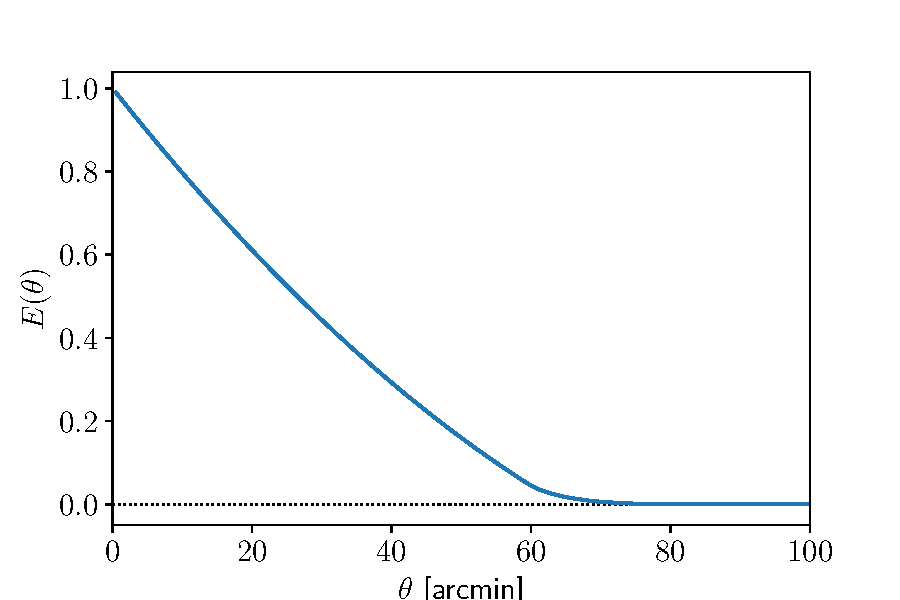
\includegraphics[width=0.7\textwidth]{eoftheta.pdf}
 \caption{Probability that a random pair of galaxies of separation $\theta$ lie in the same pointing.}
 \label{fig:eoftheta_lin}
 \end{figure}
\subsection{Modelling the shear correlation functions}
\label{sec:xipm_analytic}
For a first simple analysis we will assume that a deeper redshift distribution just yields a stronger shear signal, in the sense that the shear field for a deeper redshift distribution gets multiplied by a weight $W$. While this is not true for a 3-dimensional matter distribution, it should be valid for small variations in redshift. Additionally, we assume that a higher depth does not only lead to a stronger average shear, but also to a higher galaxy number density, implying a correlation between those two quantities.

Let $N^i(\b \theta),N^j(\b\theta)$ be the average weighted number of galaxies per pointing in redshift bins $i$ and $j$ and let $W^i(\b \theta),W^j(\b\theta)$ be the weighting of average shear. The observed correlation function $\xi^{ij,\text{obs}}_\pm(\theta)$ now changes from one of constant depth $\xi_\pm^{ij,\rm{const}}(\theta)$ via (compare Eq. \ref{eq:xipm_from_data})
\begin{align}
\xi^{ij,\text{obs}}_\pm(\theta) = & \frac{\la N^i(\bth)N^j(\bthp)\gamma^{i,\rm{obs}}_{\rm t}(\bth)\gamma^{j,\rm{obs}}_{\rm t}(\bthp)\ra }{\la N^i(\bth)N^j(\bthp)\ra} \pm \frac{\la N^i(\bth)N^j(\bthp)\gamma^{i,\rm{obs}}_\times(\bth)\gamma^{j,\rm{obs}}_\times(\bthp)\ra }{\la N^i(\bth)N^j(\bthp)\ra} \nonumber\\
 = & \frac{\la N^i(\bth)N^j(\bthp)W^i(\bth)W^j(\bthp)\ra}{\la N^i(\bth)N^j(\bthp)\ra}\left( \la \gamma^i_{\rm t}(\bth)\gamma^j_{\rm t}(\bthp)\ra \pm \la \gamma^i_\times(\bth)\gamma^j_\times(\bthp)\ra \right) \nonumber\\
 = & \frac{\la N^i(\bth)N^j(\bthp)W^i(\bth)W^j(\bthp)\ra}{\la N^i(\bth)N^j(\bthp)\ra} \xi_{\pm}^{ij,\rm{const}}(\theta) \, ,
 \label{eq:xipmblub1}
 \end{align}
 where the average $\la\ldots\ra$ represents both an ensemble average as well as an average over the position $\bth$.
 Assuming that depth and galaxy number density of neighbouring pointings are uncorrelated, the only important property of a galaxy pair is whether or not they lie in the same pointing, which is described by the function $E(\theta)$.

To compute the modified shear correlation functions, we parametrize the number densities \linebreak$N^{i}(\b \theta)=\la N^{i} \ra [1+n^{i}(\b \theta)]$ and the weight $W^{i}(\b \theta)=1+w^{i}(\b \theta)$ and, as in \eqref{eq:defweightf}, interpret $n^{i}(\b \theta)$ as a function with average $\la n^{i} \ra = 0$, that is constant on each pointing. Inspecting Eq.\,\eqref{eq:xipmblub1}, without loss of generality we can set $\la N^i\ra = 1$, as this term appears both in numerator and denominator. We can see that $\la n^i(\bth)n^j(\bthp)\ra = E(\theta)\la n^i(\bth)n^j(\bth)\ra \equiv E(\theta)\la n^i n^j \ra$ holds and compute:
\begin{align}
&\la N^i(\bth)N^j(\bthp)W^i(\bth)W^j(\bthp)\ra \nonumber\\
&\qquad =  \la [1+n^i(\bth)]\,[1+n^j(\bthp)]\,[1+w^i(\bth)]\,[1+w^j(\bthp)]\ra \nonumber\\
&\qquad =  1 + \la n^i(\bth)n^j(\bthp)\ra + \la n^i(\bth)w^i(\bth)\ra + \la n^i(\bth)w^j(\bthp)\ra + \la n^j(\bthp) w^i(\bth)\ra \nonumber\\
&\qquad\quad + \la n^j(\bthp) w^j(\bthp) \ra + \la w^i(\bth)w^j(\bthp)\ra + \la n^i(\bth)n^j(\bthp)w^i(\bth)\ra \nonumber\\
&\qquad\quad + \la n^i(\bth)n^j(\bthp)w^j(\bthp)\ra  + \la n^i(\bth)w^i(\bth)w^j(\bthp)\ra + \la n^j(\bthp) w^i(\bth)w^j(\bthp)\ra \nonumber\\
&\qquad\quad + \la  n^i(\bth)n^j(\bthp)w^i(\bth)w^j(\bthp)\ra \nonumber\\
&\qquad =  1 + \la n^iw^i\ra + \la n^j w^j\ra + E(\theta)\left[ \la n^in^j\ra + \la n^i w^j \ra  + \la n^jw^i\ra + \la w^iw^j\ra + \la n^in^jw^i\ra + \la n^in^jw^j\ra + \la n^iw^iw^j\ra \right. \nonumber\\
&\qquad\quad \left. + \la n^jw^iw^j\ra + \la n^in^jw^iw^j\ra  \right] 
 \end{align}
Ignoring correlations higher than second order\footnote{Assuming $n$ and $w$ are small, this is a valid approximation. However, inspecting Figure \ref{fig:number_density_vs_redshift}, we see that this assumption is not necessarily valid. However, we performed both calculations for the KV450-survey and found no significant difference.}, and performing the same calculation for the denominator of Eq.\,\eqref{eq:xipmblub1}, we get
 \begin{align}
 \xi^{ij,\rm{obs}}_\pm(\theta) = \frac{1 + \la n^iw^i\ra + \la n^jw^j\ra + E(\theta)\left[\la n^in^j\ra + \la n^iw^j\ra + \la n^j w^i\ra + \la w^iw^j\ra\right]}{1+E(\theta)\la n^i n^j\ra }\xi^{ij,\rm{const}}_\pm (\theta) \, .
 \end{align}
We see that in addition to a modification of the correlation function due to the stronger shear signal in deeper pointings, we also get a scale-independent modification due to the correlation between depth and number density.

For the calculation of the reference correlation functions $\xi_\pm^{ij}(\theta)$ we distribute the \textit{same} galaxies into our survey, only this time we will not order their weightings $W$ or their number densities $N$ by pointing. We can imagine this by cutting the footprint into infinitesimal elements $\d^2\b\theta$, and redistributing those at random. When we calculate the correlation function of this survey, we note that $\la n^i(\bth)\ra \la n^j(\bthp)\ra = 0$ holds for $\b\theta\neq \b 0$, as the two corresponding infinitesimal elements have uncorrelated weighting and number density. We again calculate \begin{align}
\xi^{ij}_\pm(\theta) = \frac{\la N^i(\bth)N^j(\bthp)W^i(\bth)W^j(\bthp)\ra}{\la N^i(\bth)N^j(\bthp)\ra} \xi_{\pm}^{ij,\rm{const}}(\theta) \, ,
 \label{eq:referencecorr1}
\end{align}
only this time, as weight and number density between different positions are uncorrelated, the denominator of Eq.\,\eqref{eq:referencecorr1} is unity and the numerator is \[
\la [1+n^i(\bth)]\,[1+n^j(\bthp)]\,[1+w^i(\bth)]\,[1+w^j(\bthp)]\ra = 1 + \la n^iw^i\ra + \la n^j w^j\ra\, .
\]
This yields a relation between the correlation function of constant optical depth $\xi_\pm^{ij,\rm{const}}$ and the modelled one $\xi_\pm^{ij}$:
\begin{equation}
\xi_\pm^{ij}(\theta) = \left(1+\la n^iw^i\ra + \la n^jw^j\ra \right)\xi_\pm^{ij,\rm{const}}(\theta)\, .
\end{equation}
The ratio of modelled and observed correlation function thus becomes: \begin{align}
\frac{\xi^{ij}_\pm(\theta)}{\xi_\pm^{ij,\rm{obs}}(\theta)} = & \frac{\left(1+\la n^iw^i\ra+\la n^jw^j\ra \left)\left(1+E(\theta)\la n^in^j\ra\right)\right.\right.}{1 + \la n^iw^i\ra + \la n^jw^j\ra + E(\theta)\left[\la n^in^j\ra + \la n^iw^j\ra + \la n^j w^i\ra + \la w^iw^j\ra\right]} \nonumber\\[10pt]
\approx & \frac{1+\la n^iw^i\ra+\la n^jw^j\ra + E(\theta)\la n^in^j\ra}{1 + \la n^iw^i\ra + \la n^jw^j\ra + E(\theta)\left[\la n^in^j\ra + \la n^iw^j\ra + \la n^j w^i\ra + \la w^iw^j\ra\right]}
\, .
\end{align}
It is interesting to note that $\xi^{ij}_\pm = \xi_\pm^{ij,\rm{obs}}$ holds wherever $E(\theta)=0$, meaning that the correlation function is not affected for large angular scales. Given a set of average redshifts, following \citet{2006APh....26...91V}, we can estimate 
\[
\la |\gamma| \ra \propto \la z \ra ^{0.85}\, .
\]
We shall later see that this approximation is valid for higher tomographic redshift bins $z\gtrsim 0.5$, but starts to break down at lower redshifts. We thus want to construct a model that is valid for an arbitrary distribution of redshifts and does not rely on the assumption of a single lens plane. 

\section{Semi-analytical model for the shear correlation functions}
\label{sec:xipm_semianalytic}
The analysis of data from the Kilo-Degree Survey showed that the redshift-distribution of sources was highly correlated with the depth in the $r$-band. We thus chose to separate the survey into 10 percentiles, sorted by $r$-band depth, meaning that if a pointing had a worse depth than 90\% of the other pointings, it would belong to the first percentile, and so on. Now for each percentile $m$ and each tomographic redshift bin $i$ we can extract a weighted number of galaxies $N^i_m$ and, in case the pointing overlaps with a spectroscopic survey, a source redshift distribution $p^i_m(z)$. Using \eqref{eq:xipm_from_pkappa}, we can compute the shear correlation functions $\xi_{\pm,mn}^{ij}(\theta)$ for each set of percentiles $m,n$ and redshift bins $i,j$\footnote{For the calculation of the shear correlation functions we use the \textsc{Nicaea}-program. Among other things, it calculates the shear correlation functions for a given cosmology and source redshift distribution. To estimate the power spectrum on nonlinear scales we use the methods developed by \citet{2012ApJ...761..152T}.}. When we compute the measured shear correlation functions of a survey, we take the weighted average of tangential and cross shears of all pairs of galaxies (\citet{2017MNRAS.465.1454H} give a good overview for the process). If, for a single pair of galaxies, one galaxy lies in the $m$-th percentile of redshift bin $i$ and the second one lies in the $n$-th percentile of redshift bin $j$, then their contribution to the observed correlation functions is, on average, $\xi_{\pm,mn}^{ij}(\theta)$. This means that if we know each of those single correlation functions, we can reconstruct the total correlation functions via a weighted average of the single functions. Formally, we define \[
\xi_\pm^{ij,\rm{obs}}(\theta) = \frac{\sum_{m,n} P_{mn}^{ij}(\theta)\xi_{\pm,mn}^{ij}(\theta)}{\sum_{m,n} P_{mn}^{ij}(\theta)}\, ,
\label{eq:def_xiobs}
\]
where $P_{mn}^{ij}$ is the new weighting of the correlation functions. This weighting has to be proportional to the probability that a galaxy pair of distance $\theta$ is of percentiles $m$ and $n$, as well as to the original weighting of these galaxies.

For $m\neq n$ we know that the pair of galaxies has to lie in different pointings, which is accounted for by including the factor $[1-E(\theta)]$. Furthermore, the first galaxy has to lie in percentile $m$, the probability of which we will denote with $P(m)$. As we have 10 different percentiles, and average over the whole footprint of the survey, $P(m)=1/10$ holds. When the first pointing is of percentile $m$, we want to denote the probability that a galaxy in a different pointing with distance $\theta$ is of percentile $n$ by $P(n|m,\theta)$. The impact of such a galaxy pair on the correlation functions scales with the product of the weighted number of galaxies $N_m^i,N_n^j$. We get for $n\neq m$: \[
P_{mn}^{ij}(\theta) = [1-E(\theta)]\frac{1}{10}P(n|m,\theta) N_m^i N_n^j\, .
\label{eq:pmnij_corr1}
\]
For the calculation of $P_{mm}^{ij}(\theta)$ we have to account for a different possibility: In case that the galaxy lies in the same pointing [accounted for by the factor $E(\theta)$], it automatically is of the same percentile. We therefore set \[
P_{mm}^{ij}(\theta) = E(\theta)\frac{1}{10} N_m^iN_m^j + [1-E(\theta)]\frac{1}{10}P(m|m,\theta) N_m^i N_m^j \, .
\label{eq:pmnij_corr2}
\]
In our case, we assume an uncorrelated distribution of percentiles, such that we can set $P(n|m,\theta)=1/10$. We can then write $P_{mn}^{ij}(\theta)$ as: \[
P_{mn}^{ij}(\theta) = E(\theta)\frac{1}{10} N_m^iN_n^j\,\delta_{mn} + [1-E(\theta)]\frac{1}{100} N_m^i N_m^j \, ,
\label{eq:pmnij_uncorr}
\]
where $\delta_{mn}$ denotes the Kronecker delta.
Inserting this into Eq.\,\eqref{eq:def_xiobs}, we compute
\begin{align}
\xi_{\pm,mn}^{ij,\rm{obs}}(\theta) = & \frac{1}{C}\sum_{m=1}^{10} N_m^i \bigg\{ E(\theta) N_m^j \xi_{\pm,mm}^{ij}(\theta) + \frac{\big[1-E(\theta)\big]}{10}\sum_{n=1}^{10}N_n^j \xi_{\pm,mn}^{ij}(\theta)\bigg\}\, ,
\label{eq:correctionfunction1}
\end{align}
with the normalization
\[
C = \sum_{m=1}^{10} N_m^i \bigg[ E(\theta)  N_m^j + \frac{\big[1-E(\theta)\big]}{10}\sum_{n=1}^{10} N_n^j\bigg]\, .
\]
A more mathematically rigorous derivation of this function can be found in Appendix \ref{sec:calc of xipm}.

If we want to compute this for all 5 redshift bins of the KV450-survey, this forces us to calculate 1275 correlation functions and add them, thus yielding potential numerical errors (apart from being computationally expensive). However, if we examine Eq.\,\eqref{eq:lens_efficiency}, we see that the comoving distance distribution of sources factors in linearly. This in turn implies that in Equations \eqref{eq:pkappa} and \eqref{eq:xipm_from_pkappa} both source distance distributions factor in linearly. This basically means that, instead of adding correlation functions, we can add their respective redshift distributions and compute the correlation functions of that. In particular, we can define the \textit{combined number of galaxies} $N^i$ and \textit{average redshift distribution} $p^i(z)$ of tomographic bin $i$ as \[
N^i\equiv\sum_m N_m^i\, , \qquad p^i(z) = \frac{\sum_m N_m^i p_m^i(z)}{\sum_m N_m^i} \, .
\]
If we define $\xi^{ij}_\pm$ as the correlation functions between the average redshift distributions $p^i(z)$ and $p^j(z)$, then we observe: \[
\sum_{m,n}N_m^iN_n^j\xi^{ij}_{\pm,mn} = N^iN^j\xi^{ij}_\pm\, .
\]
Consequently, we can apply this to \eqref{eq:correctionfunction1}, yielding
\begin{equation}
\xi_{\pm}^{ij,\rm{obs}}(\theta) = \frac{1}{C}\bigg\{ E(\theta)\left[\sum_{m=1}^{10} N_m^iN_m^j \xi_{\pm,mm}^{ij}(\theta)\right] +\frac{\big[1-E(\theta)\big]}{10}\xi_\pm^{ij}(\theta)N^iN^j\bigg\}\, .
\label{eq:correctionfunction2}
\end{equation}
For each set of redshift bins we thus only have to compute eleven correlation functions, which reduces the number of functions to compute from 1275 to 165. We can see that for large distances $\theta$, such that $E(\theta)=0$ holds, we have $C=N^iN^j$ and thus \[
\xi_{\pm}^{ij,\rm{obs}}(\theta) = \frac{1}{N^iN^j}\xi_\pm^{ij}(\theta)N^iN^j = \xi_\pm^{ij}(\theta)\, ,
\]
so on large scales our observed correlation functions agree with the ones that we would usually calculate.

%%% Local Variables: 
%%% mode: latex
%%% TeX-master: "../mythesis"
%%% End: 